\section{Results and Discussion}
\subsection{Main Results}
Table \ref{tab:pump_performance_summary} shows the experimental and manufacturer pump performance summary. The pump configuration, valve configuration, pump speed, volumetric flow rate, corrected head, head coefficient, and flow coefficient are shown. Sample calculations for the single pump in Appendix \ref{sec:single_pump_analysis}. Parallel and series pump performance analysis is shown in Appendix \ref{sec:parallel_and_series_pump_analysis}.
\begin{longtable}{p{0.10\textwidth}p{0.15\textwidth}C{0.08\textwidth}C{0.12\textwidth}C{0.08\textwidth}C{0.12\textwidth}C{0.12\textwidth}}
    \caption{Experimental and Manufacturer Pump Performance Summary} \\
    \label{tab:pump_performance_summary} \\[-8ex]
    \toprule
    Pump Config. & Valve Config. & Pump Speed, $\Omega$ & Volumetric Flow Rate, $Q$ & Corrected Head, $H$ & Head Coefficient, $\Psi$ & Flow Coefficient, $\Phi$ \\
    & & ($\unit{\rpm}$) & ($\unit{\meter\cubed\per\second}$) & ($\unit{\meter}$) & & \\
    \midrule
    Single & Fully open & 1800 & 0.003159 & 2.91 & 0.275 & 0.12 \\
    Single & Partial 1 & 1800 & 0.003003 & 3.16 & 0.300 & 0.11 \\
    Single & Partial 2 & 1800 & 0.001492 & 5.09 & 0.482 & 0.05 \\
    Single & Closed & 1800 & - & 5.49 & 0.520 & 0.00 \\
    Single & Fully open & 2700 & 0.004858 & 5.91 & 0.249 & 0.12 \\
    Single & Partial 1 & 2700 & 0.004749 & 6.31 & 0.265 & 0.12 \\
    Single & Partial 2 & 2700 & 0.002911 & 10.6 & 0.445 & 0.07 \\
    Single & Closed & 2700 & - & 12.4 & 0.522 & 0.00 \\
    Single & Fully open & 3600 & 0.006474 & 9.72 & 0.230 & 0.12 \\
    Single & Partial 1 & 3600 & 0.006240 & 11.2 & 0.266 & 0.11 \\
    Single & Partial 2 & 3600 & 0.002454 & 20.8 & 0.491 & 0.05 \\
    Single & Closed & 3600 & - & 21.8 & 0.515 & 0.00 \\
    Single & Manufacturer & 1800 & 0.0040 & 2.58 & 0.244 & 0.15 \\
    Single & Manufacturer & 1800 & 0.0033 & 4.14 & 0.392 & 0.12 \\
    Single & Manufacturer & 1800 & 0.0026 & 4.96 & 0.470 & 0.10 \\
    Single & Manufacturer & 1800 & 0.0020 & 5.40 & 0.511 & 0.07 \\
    Single & Manufacturer & 2700 & 0.0060 & 5.77 & 0.243 & 0.15 \\
    Single & Manufacturer & 2700 & 0.0050 & 9.12 & 0.384 & 0.12 \\
    Single & Manufacturer & 2700 & 0.0040 & 11.0 & 0.463 & 0.10 \\
    Single & Manufacturer & 2700 & 0.0030 & 12.1 & 0.509 & 0.07 \\
    Single & Manufacturer & 2700 & 0.0020 & 12.8 & 0.539 & 0.05 \\
    Single & Manufacturer & 3600 & 0.0080 & 10.3 & 0.244 & 0.15 \\
    Single & Manufacturer & 3600 & 0.0067 & 16.1 & 0.381 & 0.12 \\
    Single & Manufacturer & 3600 & 0.0054 & 19.2 & 0.454 & 0.10 \\
    Single & Manufacturer & 3600 & 0.0040 & 21.6 & 0.511 & 0.07 \\
    Single & Manufacturer & 3600 & 0.0027 & 22.8 & 0.540 & 0.05 \\
    Parallel & Fully open & 2700 & 0.007266 & 11.3 & 0.474 & 0.18 \\
    Parallel & Partial 1 & 2700 & 0.006283 & 11.7 & 0.492 & 0.15 \\
    Parallel & Partial 2 & 2700 & 0.002217 & 12.5 & 0.528 & 0.05 \\
    Parallel & Closed & 2700 & - & 12.5 & 0.526 & 0.00 \\
    Series & Fully open & 2700 & 0.005584 & 9.15 & 0.385 & 0.14 \\
    Series & Partial 1 & 2700 & 0.005449 & 10.4 & 0.439 & 0.13 \\
    Series & Partial 2 & 2700 & 0.002983 & 21.9 & 0.921 & 0.07 \\
    Series & Closed & 2700 & - & 24.9 & 1.048 & 0.00 \\
    \bottomrule
\end{longtable}

\subsection{Single Pump Performance}
\subsubsection{Head vs. Flow Rate}
Using the data from Table \ref{tab:pump_performance_summary}, the head vs. flow rate for the experimental single pump data was plotted in Figure \ref{fig:single_pump_plot}. Error bars were shown for the volumetric flow, where time was the biggest contributor to error. This is likely due to the reaction time of the stopwatch operator causing a high precision error. The error bars for the head were much smaller and omitted for visual clarity. Calculations for the error bars are shown in Appendix \ref{sec:single_pump_analysis}. 
\begin{figure}[H]
    \centering
    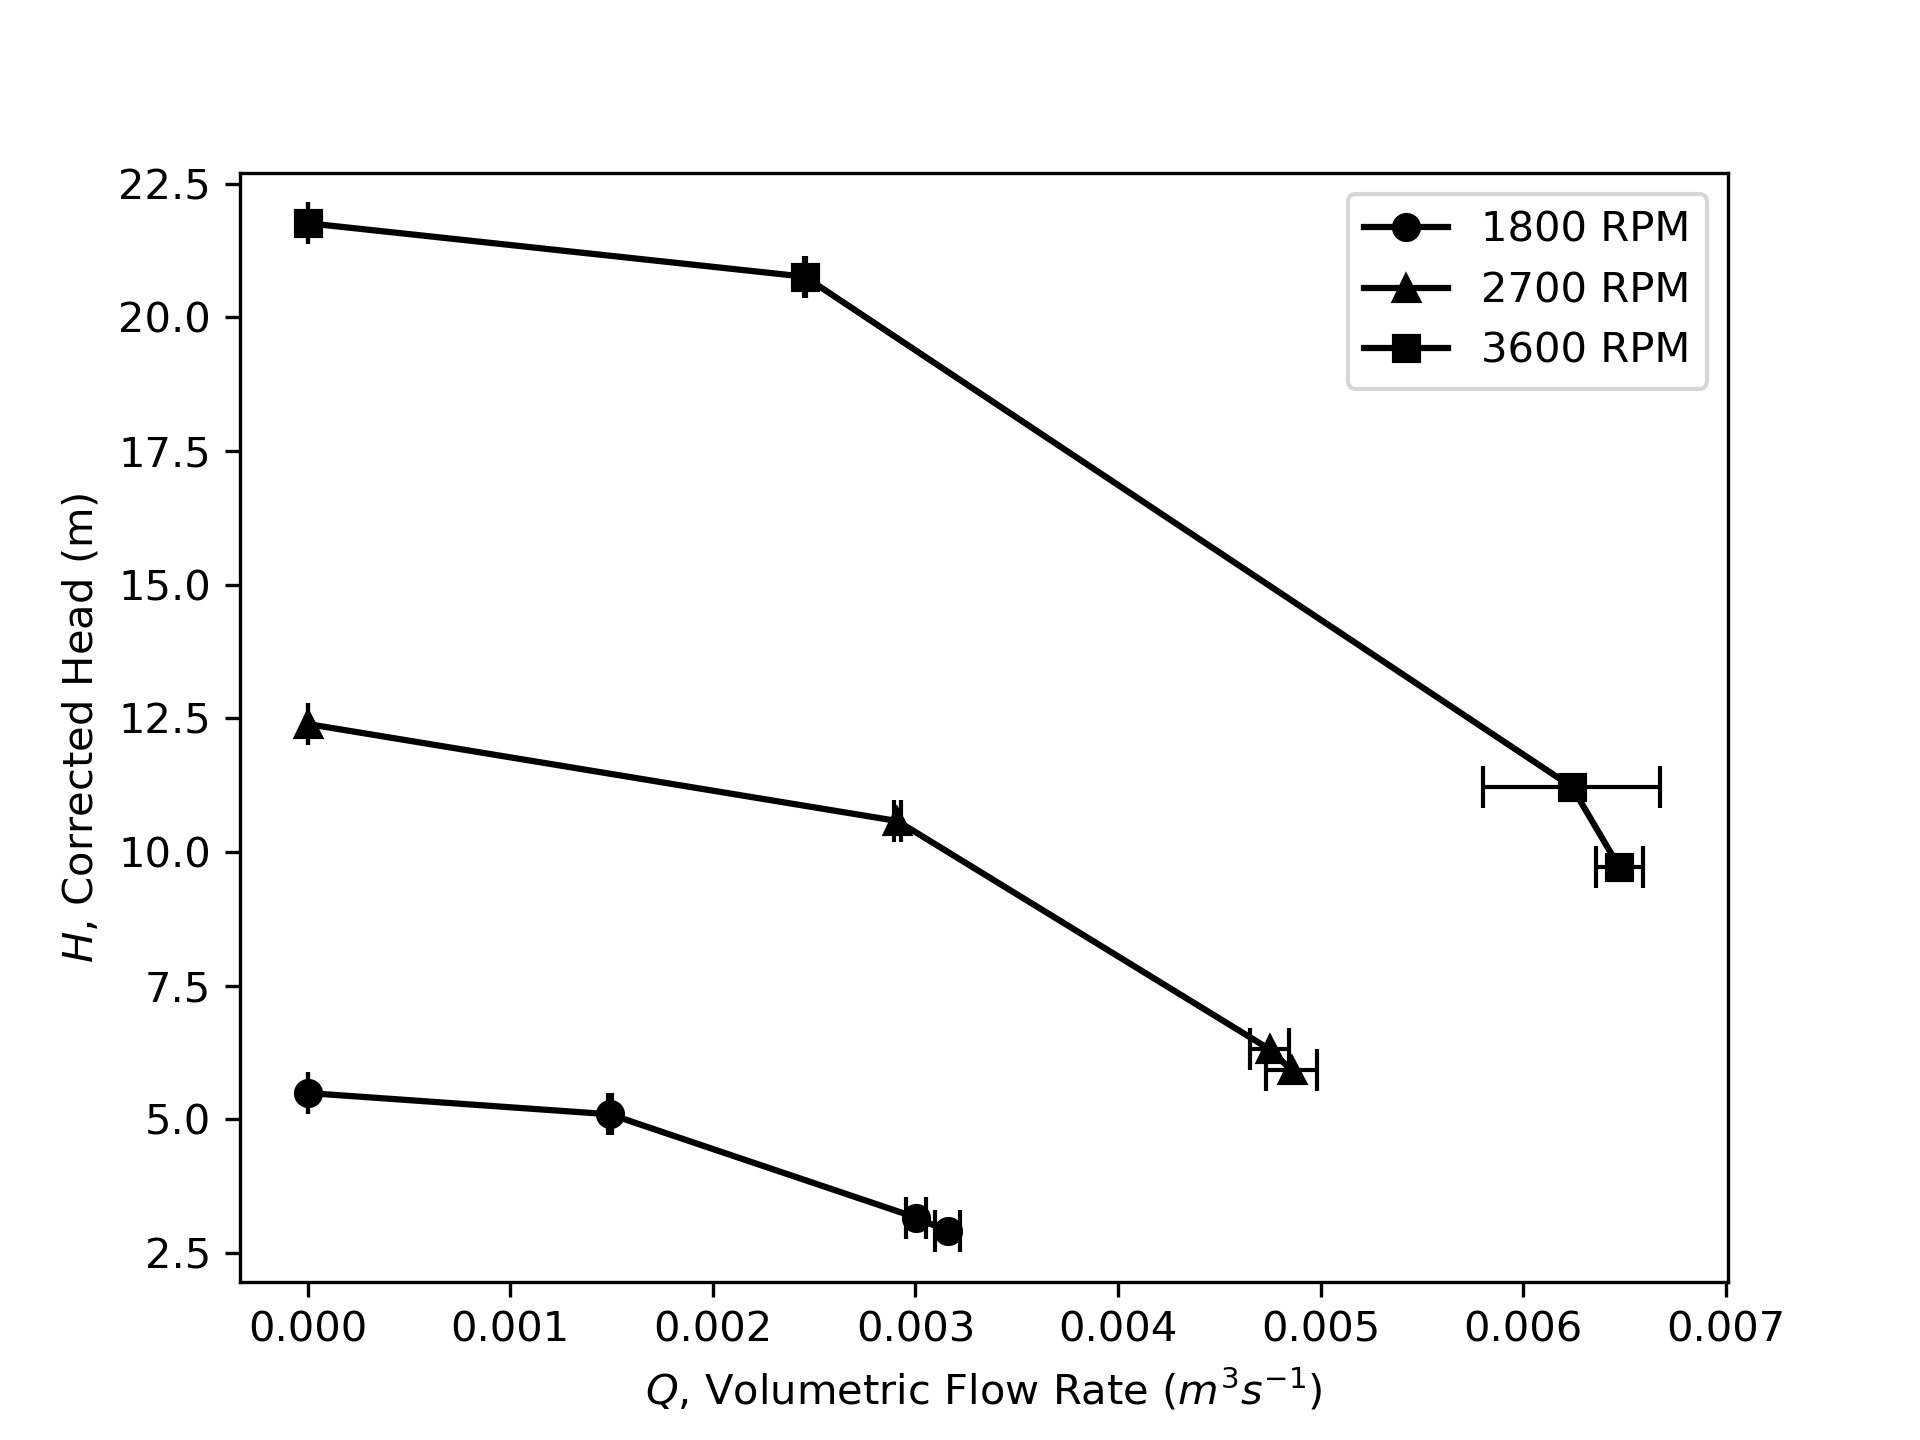
\includegraphics[width=0.5\textwidth]{Sections/Figures/Single Pump Plot.png}
    \caption{Single pump experimental head vs. flow rate plot.}
    \label{fig:single_pump_plot}
\end{figure}

\subsubsection{Head Coefficient vs. Flow Coefficient}
The head coefficient and flow coefficient for the experimental, manufacturer, and ideal pump data are shown in Figure \ref{fig:single_pump_coefficients_plot}. The ideal pump data was calculated from ideal pump equation (Eq. \ref{ideal_turbo_machinary}) using the impeller angle. Impeller angle was determined visually, shown in Appendix \ref{sec:impeller_angle}. Sample calculations for the experimental and manufacturer head and flow coefficients are shown in Appendix \ref{sec:single_pump_analysis}.

For the single experimental pump, the head and flow coefficients appear to fall onto the same curve. A non-linear relationship is observed, where the head coefficient decreases as the flow coefficient increases. Most points of different speeds are within error bars of each other. This suggests that the head and flow coefficients are independent of pump speed. The largest source of error was the precision error caused by the reaction time of the stopwatch operator.

The manufacturer head and flow coefficients also appear to fall onto the same, but different than the experimental, curve. At 3600 RPM, $Phi = 0.12$, the error between the experimental and manufacturer was 39.7\%. In general manufacturer head coefficient is higher than the experimental head coefficient for the same flow coefficient. This suggests that the manufacturer has over rated their pump.

The ideal head and flow coefficients are shown as a straight line. The ideal head coefficient is much higher than the experimental and manufacturer head coefficient for the same flow coefficient. The ideal pump neglects all losses and is overly optimistic. The linear trend does not follow the experimental and manufacturer data.
\begin{figure}[H]
    \centering
    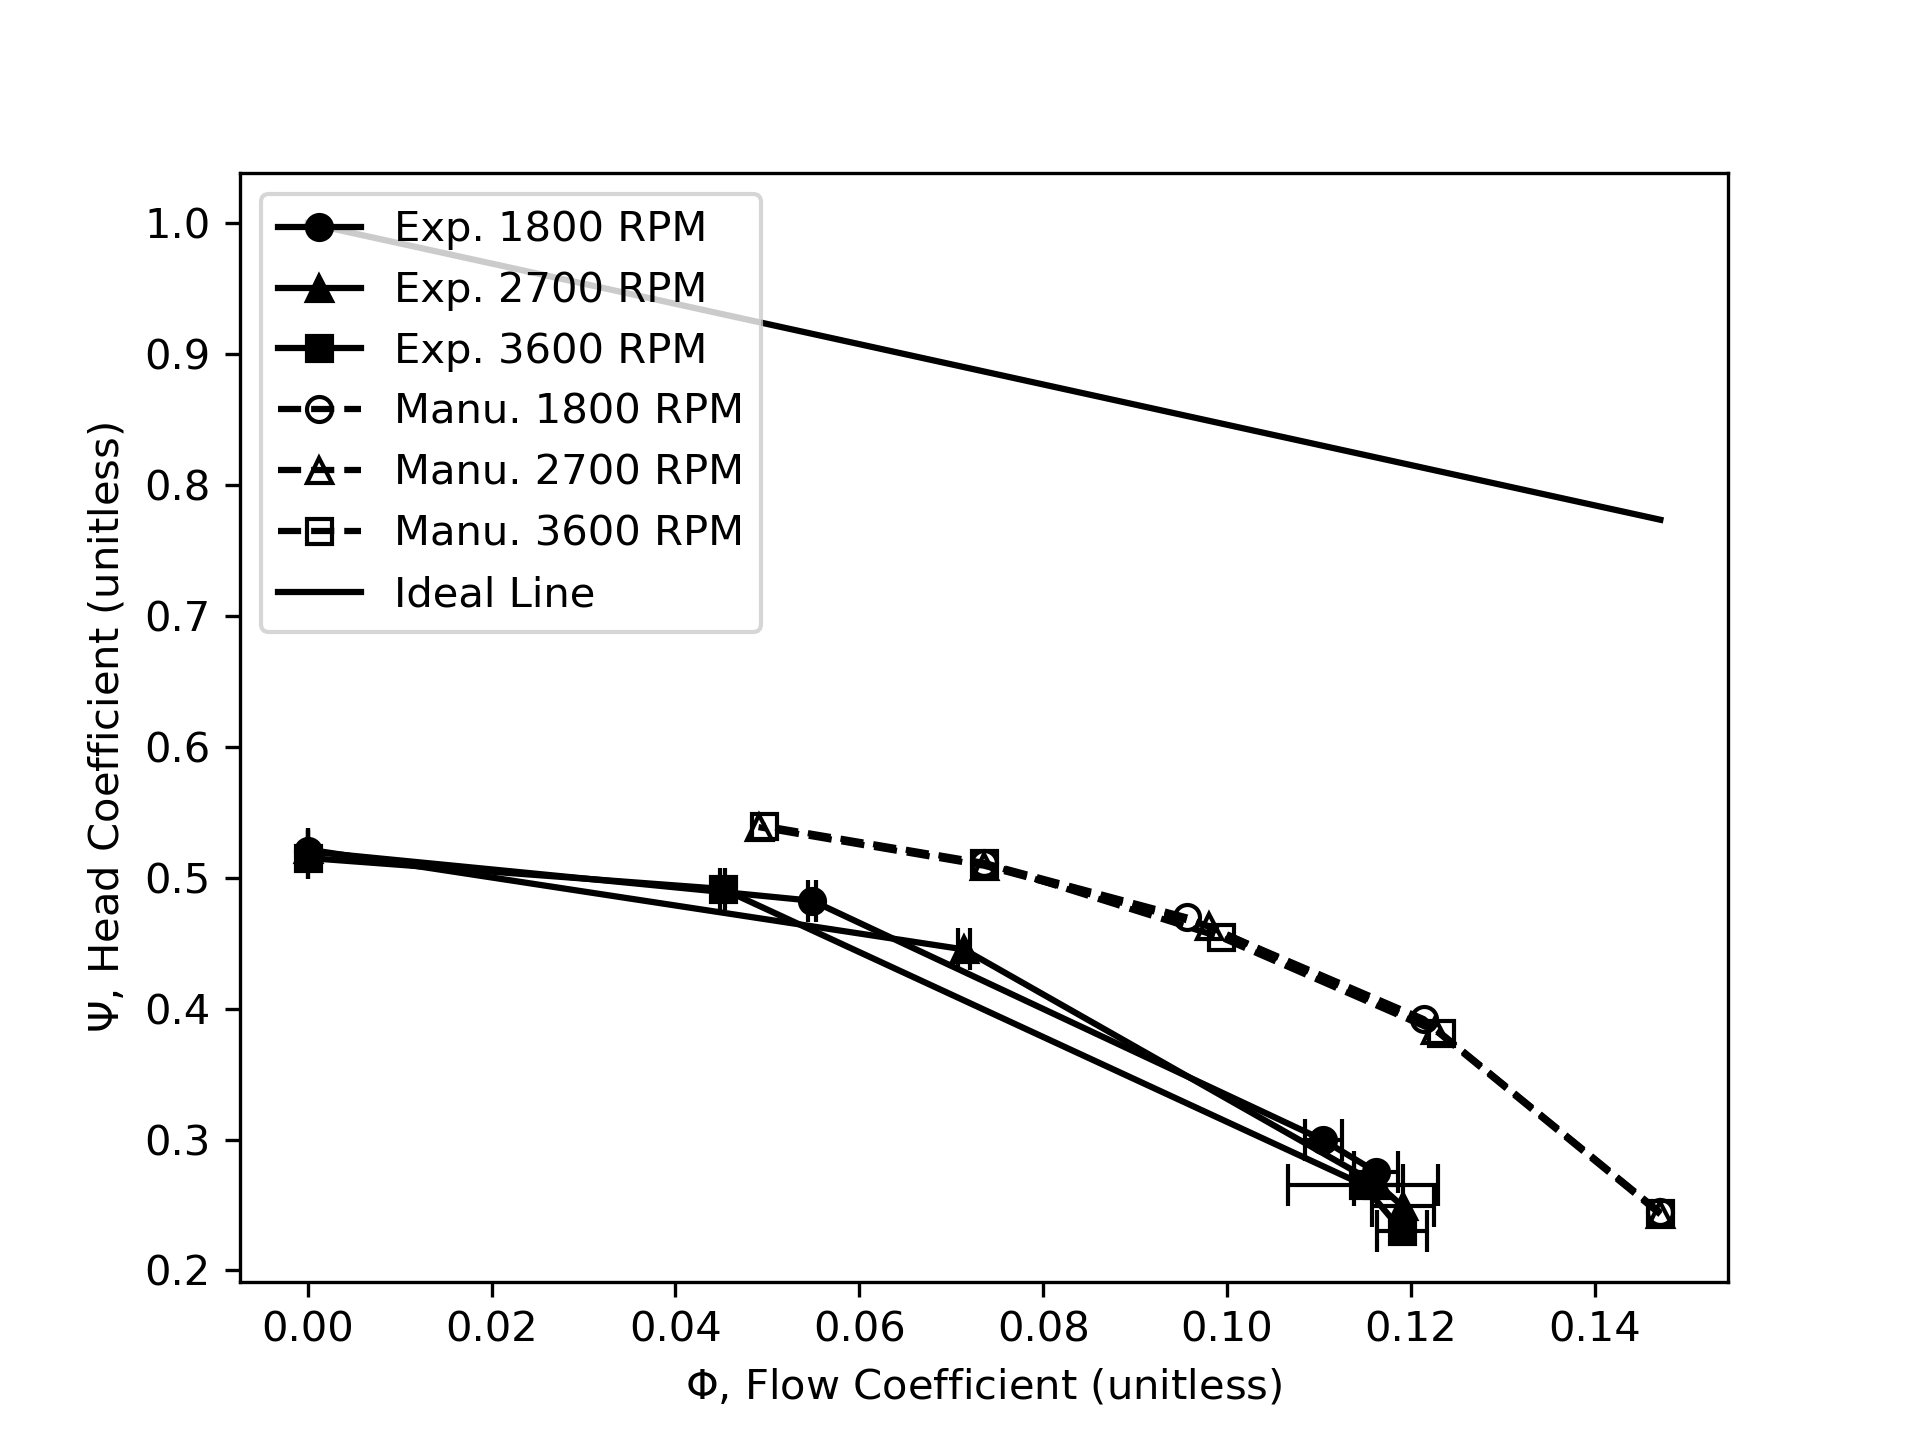
\includegraphics[width=0.6\textwidth]{Sections/Figures/Single Pump Coefficients Plot.png}
    \caption{Single pump experimental, manufacturer, and ideal head coefficient vs. flow coefficient plot.}
    \label{fig:single_pump_coefficients_plot}
\end{figure}

\subsubsection{Ideal and Rule of Thumb Shutoff Head}
\begin{longtable}{C{0.15\textwidth}C{0.15\textwidth}C{0.15\textwidth}}
    \caption{Ideal, rule of thumb, and experimental shutoff head for the single pump at 3600 $\unit{\rpm}$.} \\
    \label{tab:shutoff_head} \\[-8ex]
    \toprule
    Ideal Shutoff Head, $H'_{\text{ideal}}$ & Rule of Thumb Shutoff Head, $H'_{\text{thumb}}$ & Experimental Shutoff Head, $H'_{\text{exp}}$ \\
    ($\unit{\meter}$) & ($\unit{\meter}$) & ($\unit{\meter}$) \\
    \midrule
    42.2 & 21.1 & 21.8 \\
    \bottomrule
\end{longtable}

\noindent The ideal and rule of thumb shutoff head for the single pump at 3600 $\unit{\rpm}$ was calculated and compared to the experimental shutoff head (single closed valve configuration). The ideal and rule of thumb shutoff head was calculated using Eq. \ref{eq:ideal_shutoff_head} and \ref{eq:thumb_head}. The experimental shutoff head was taken from Table \ref{tab:pump_performance_summary}. Sample calculations for the ideal and rule of thumb shutoff head are shown in Appendix \ref{sec:shut_off_head} and the experimental shutoff head in Appendix \ref{sec:single_pump_analysis}.

The ideal shutoff head assumes all kinetic energy is lost too friction and is overly optimistic. The error was calculated to be 48.3\%. This suggests poor agreement between the experimental and ideal shutoff head.

The rule of thumb shutoff head is a more realistic estimate and is within 3.3\% of the experimental shutoff head. This suggests good agreement between the experimental and rule of thumb shutoff head.

\subsection{Parallel and Series Pump Performance}
The head vs. flow rate for the experimental parallel and series pump data was plotted in Figure \ref{fig:parallel_pump_plot} and \ref{fig:series_pump_plot}.
Error bars were shown for the volumetric flow, where time was the biggest contributor to error. This is likely due to the reaction time of the stopwatch operator causing a high precision error. The error bars for the head were much smaller and omitted for visual clarity. Sample calculations are shown in Appendix \ref{sec:parallel_and_series_pump_analysis}.

The parallel curves have poor agreement. The theoretical head was higher than the experimental head for the same flow. In addition, a higher flow was observed at the full open valve configuration. This suggests the theoretical model does not accurately predict the parallel pump performance.
\begin{figure}[H]
    \centering
    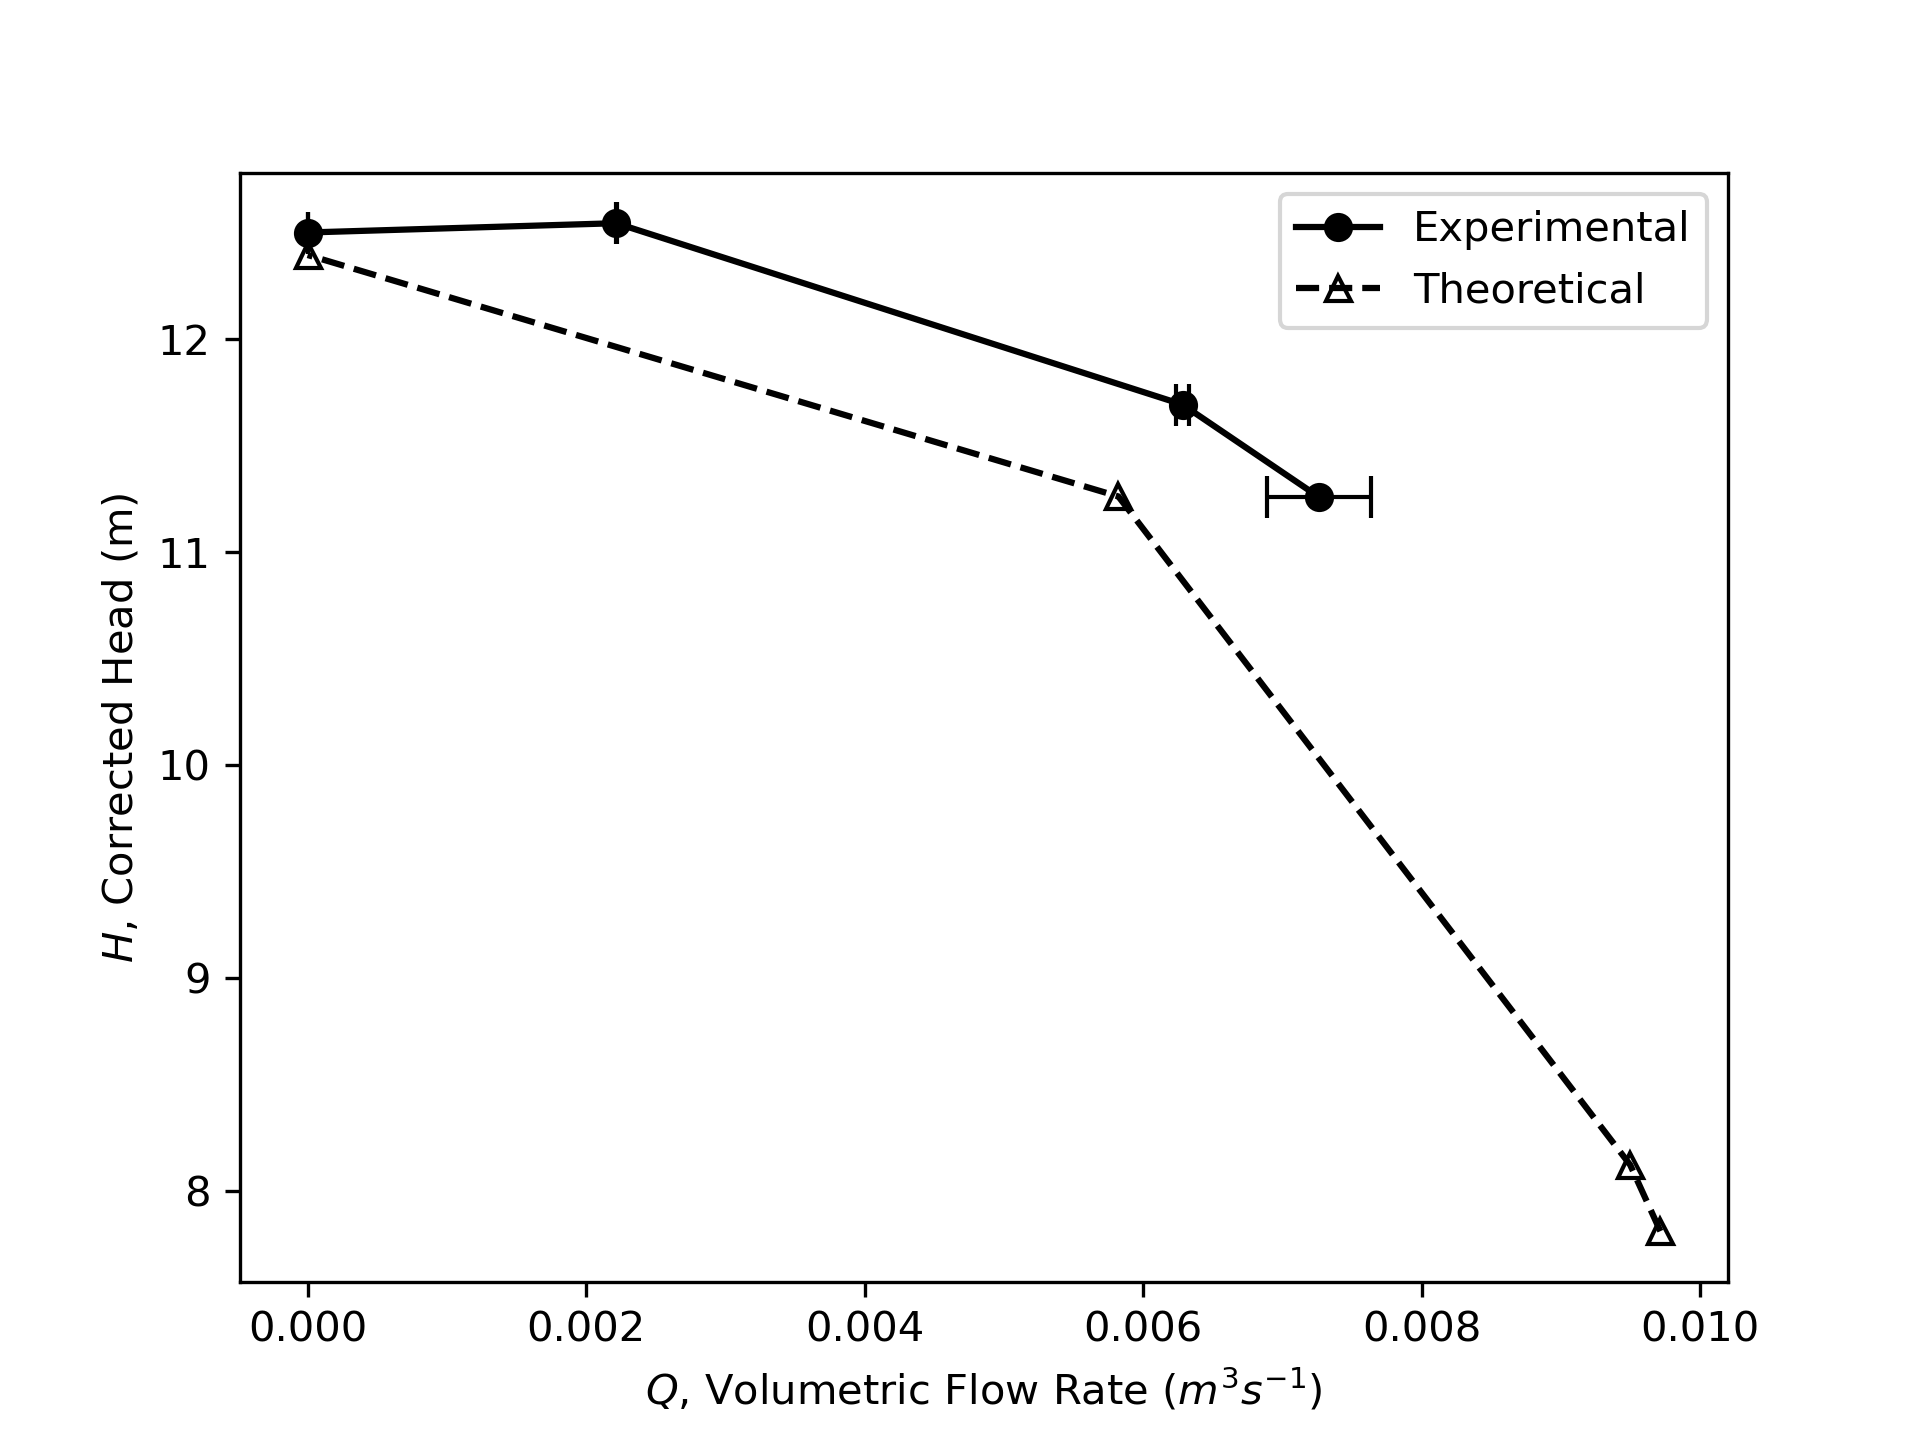
\includegraphics[width=0.5\textwidth]{Sections/Figures/Parallel Pump Plot.png}
    \caption{Parallel pump experimental and theoretical head vs. flow rate plot.}
    \label{fig:parallel_pump_plot}
\end{figure}

The series curves have some agreement. The theoretical head was lower than the experimental head for the same flow. In addition, a higher flow was observed at the full open valve configuration. These deviations were smaller than the parallel pump. This suggests the theoretical model does somewhat accurately predicts the series pump performance.

\begin{figure}[H]
    \centering
    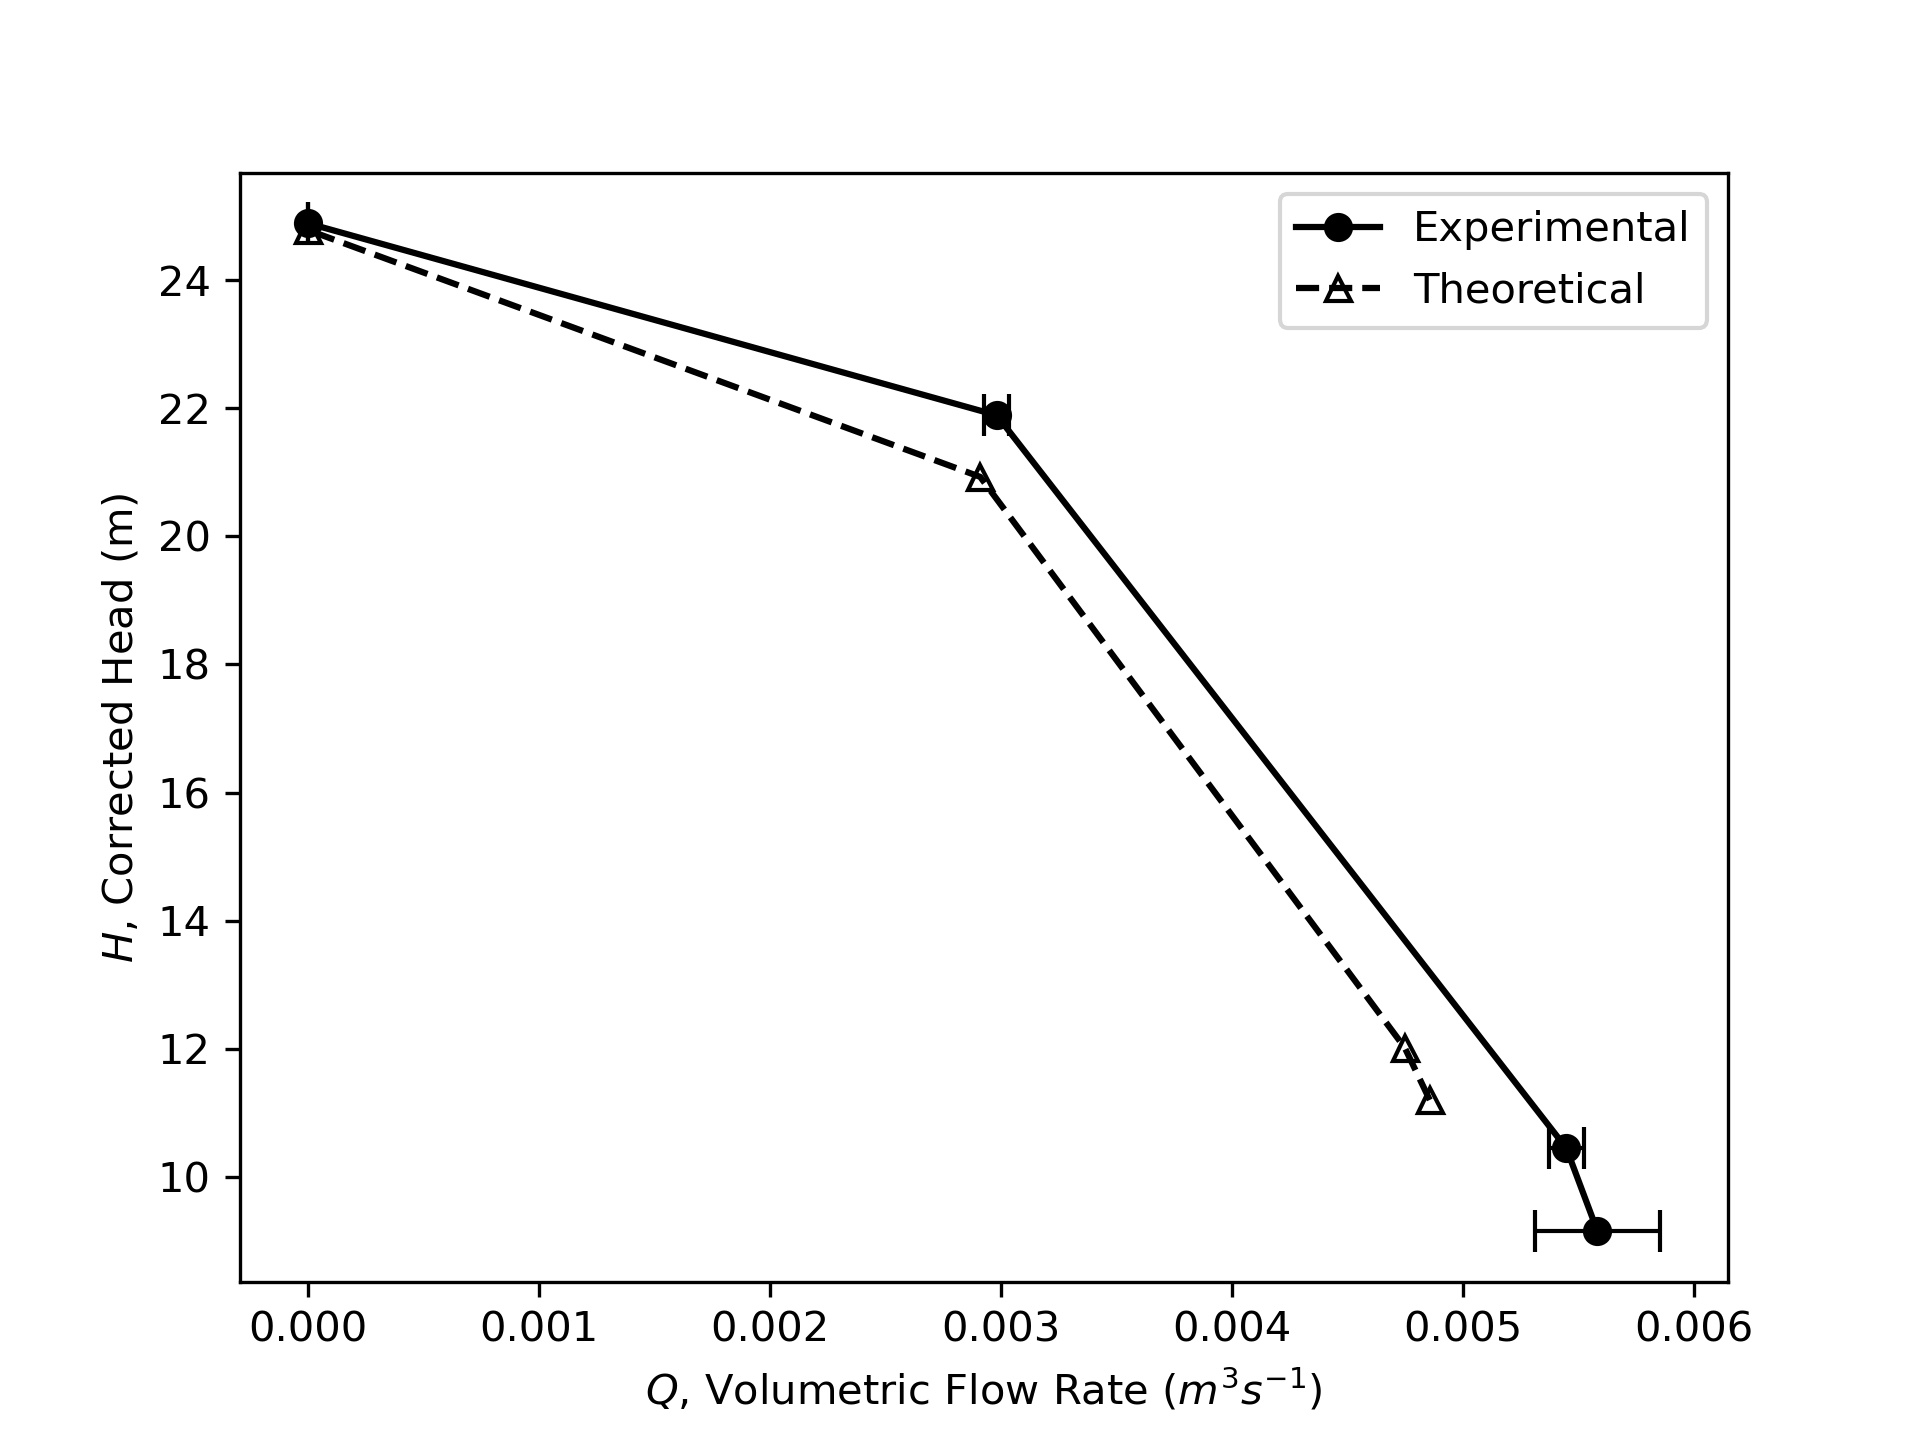
\includegraphics[width=0.5\textwidth]{Sections/Figures/Series Pump Plot.png}
    \caption{Series pump experimental and theoretical head vs. flow rate plot.}
    \label{fig:series_pump_plot}
\end{figure}

\subsection{Geometric Similarity in Manufacturer's Specifications}
The manufacturer's specifications are for geometrically dissimilar pumps. To investigate the effects of assuming similar geometry, two plots were produced. Sample calculations for the head and flow coefficients are shown in Appendix \ref{sec:geometrically_similar_pumps}.

The first plot, Figure \ref{fig:geometric_similarity_head_coefficient}, shows the head coefficient vs. flow coefficient for geometrically similar pumps where impeller blade height, $b$, and impeller width, $w$, were scaled by the impeller diameter, $D$. An observation is that the head coefficient decreases for a given flow coefficient as the impeller diameter decreases.  

The second plot, Figure \ref{fig:geometric_dissimilarity_head_coefficient}, shows the head coefficient vs. flow coefficient for geometrically dissimilar pumps where impeller blade height, $b$, and impeller width, $w$, were not scaled by the impeller diameter, $D$. An observation is that the head coefficient decreases for a given flow coefficient as the impeller diameter decreases. 

The head and flow coefficients for the geometrically similar pumps fall only somewhat collapse onto the same curve. At low flow coefficients, the head coefficient decreases as the impeller diameter decreases. For higher flow coefficients, the head coefficient increases as the impeller diameter decreases. This is not expected as the curves should collapse onto the same curve. 
The head and flow coefficients for the geometrically dissimilar pumps fall more so onto the same curve. The same trend where at low flow coefficients, the head coefficient decreases for a given flow coefficient as the impeller diameter decreases and for higher flow coefficients, the head coefficient increases for a given flow coefficient as the impeller diameter decreases. This trend is much less pronounced. This suggests that the pumps are geometrically dissimilar, which is consistent with the manufacturer's specifications.
\begin{figure}[H]
    \centering
    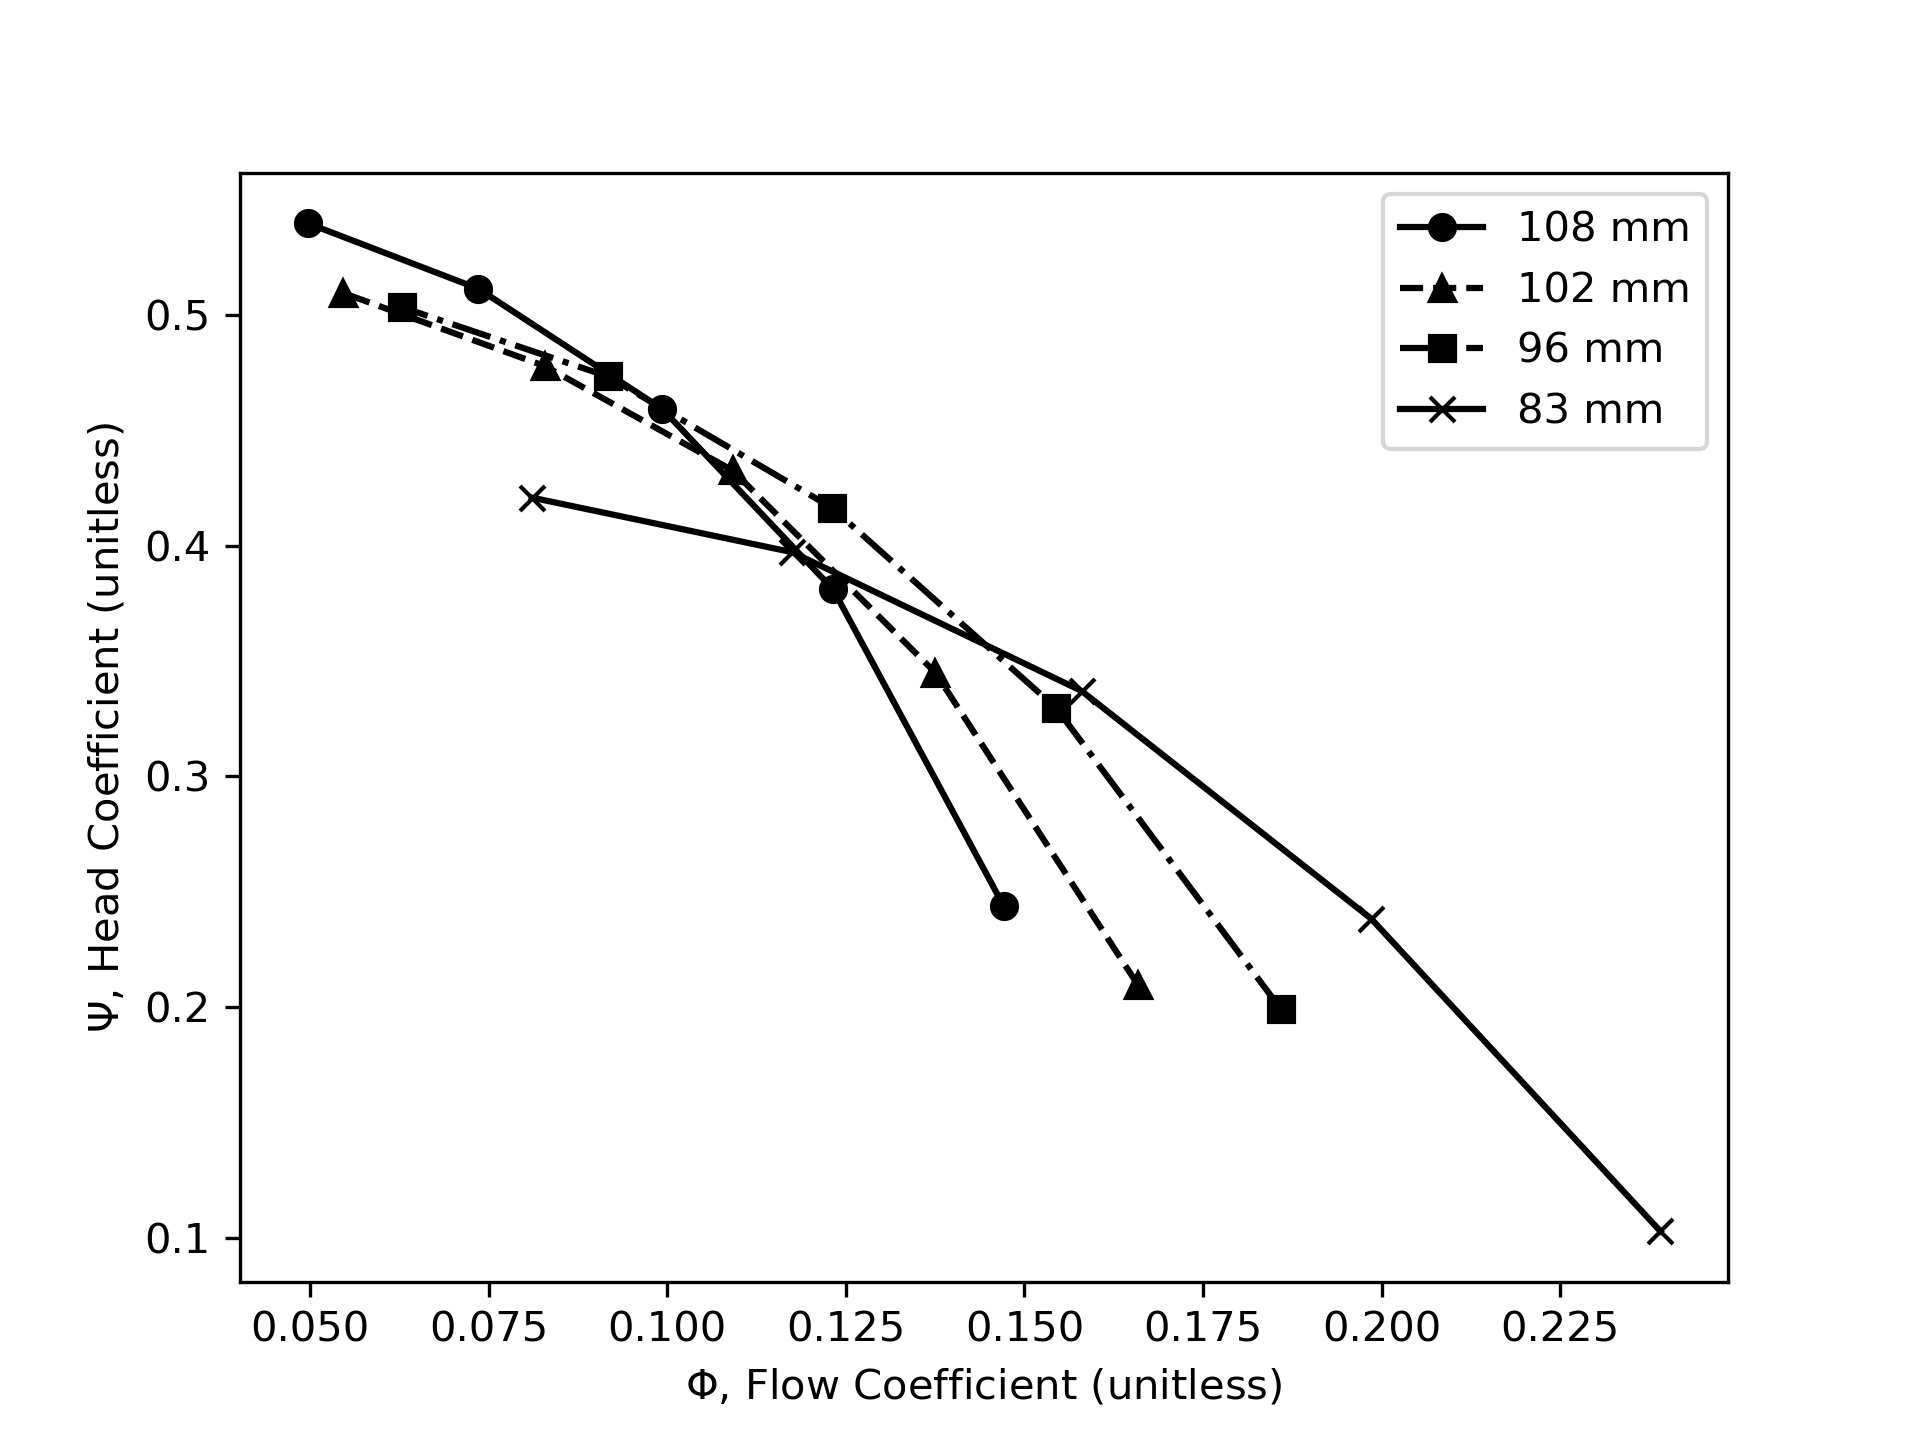
\includegraphics[width=0.5\textwidth]{Sections/Figures/Geometrically Similar Pump Coefficients Plot.png}
    \caption{Head coefficient vs. flow coefficient for geometrically similar pumps.}
    \label{fig:geometric_similarity_head_coefficient}
\end{figure}
\begin{figure}[H]
    \centering
    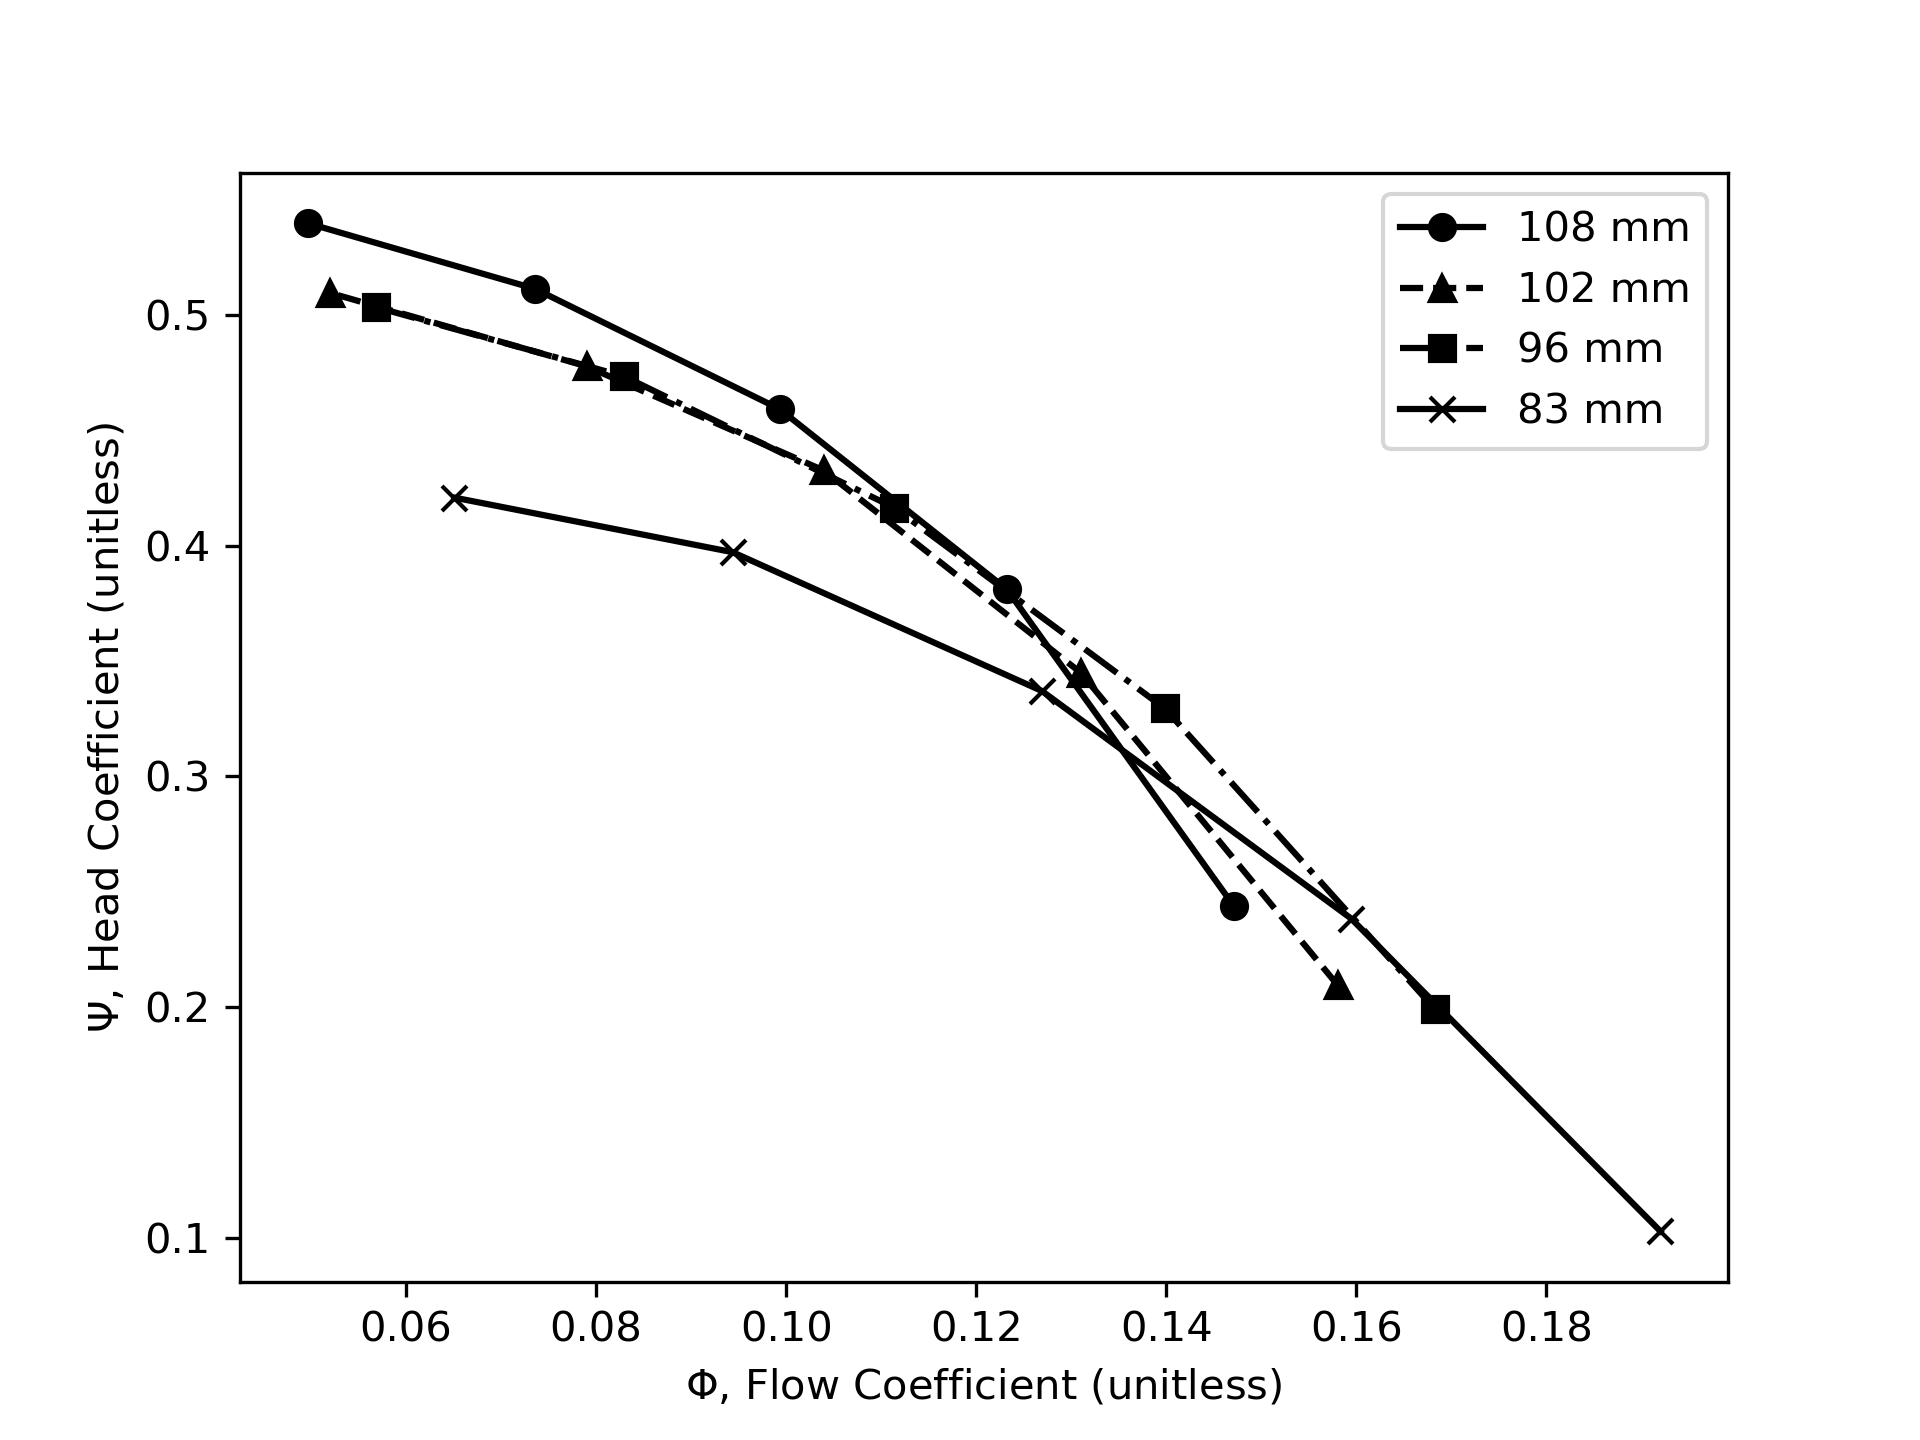
\includegraphics[width=0.5\textwidth]{Sections/Figures/Geometrically Dissimilar Pump Coefficients Plot.png}
    \caption{Head coefficient vs. flow coefficient for geometrically dissimilar pumps.}
    \label{fig:geometric_dissimilarity_head_coefficient}
\end{figure}

\subsection{Pump Efficiency}
The pump efficiencies for the experimental data was calculated in Appendix \ref{sec:pump_efficiency}. The pump effiecncies for the manufacturer data was given in the manufacturer's specifications. The plot of the experimental and manufacturer pump efficiencies is shown in Figure \ref{fig:single_pump_efficiency_plot}.

The pump had the highest efficiency of 49.9\% when operating at 2700 $\unit{\rpm}$ in a partially closed valve configuration. The pump had the lowest efficiency of 37.0\% when operating at 1800 $\unit{\rpm}$ in a partially closed valve configuration. 

The actual pump efficiency was lower than the manufacturer pump efficiency for all pump speeds. It was difficult to compare directly since the flow coefficients of the experimenal and manufacturer seldom matched. The largest deviation was approximately 29\% at 1800 $\unit{\rpm}$ and a flow coefficient of 0.12. Again, this suggests the manufacturer has over rated their pump.
\begin{figure}[H]
    \centering
    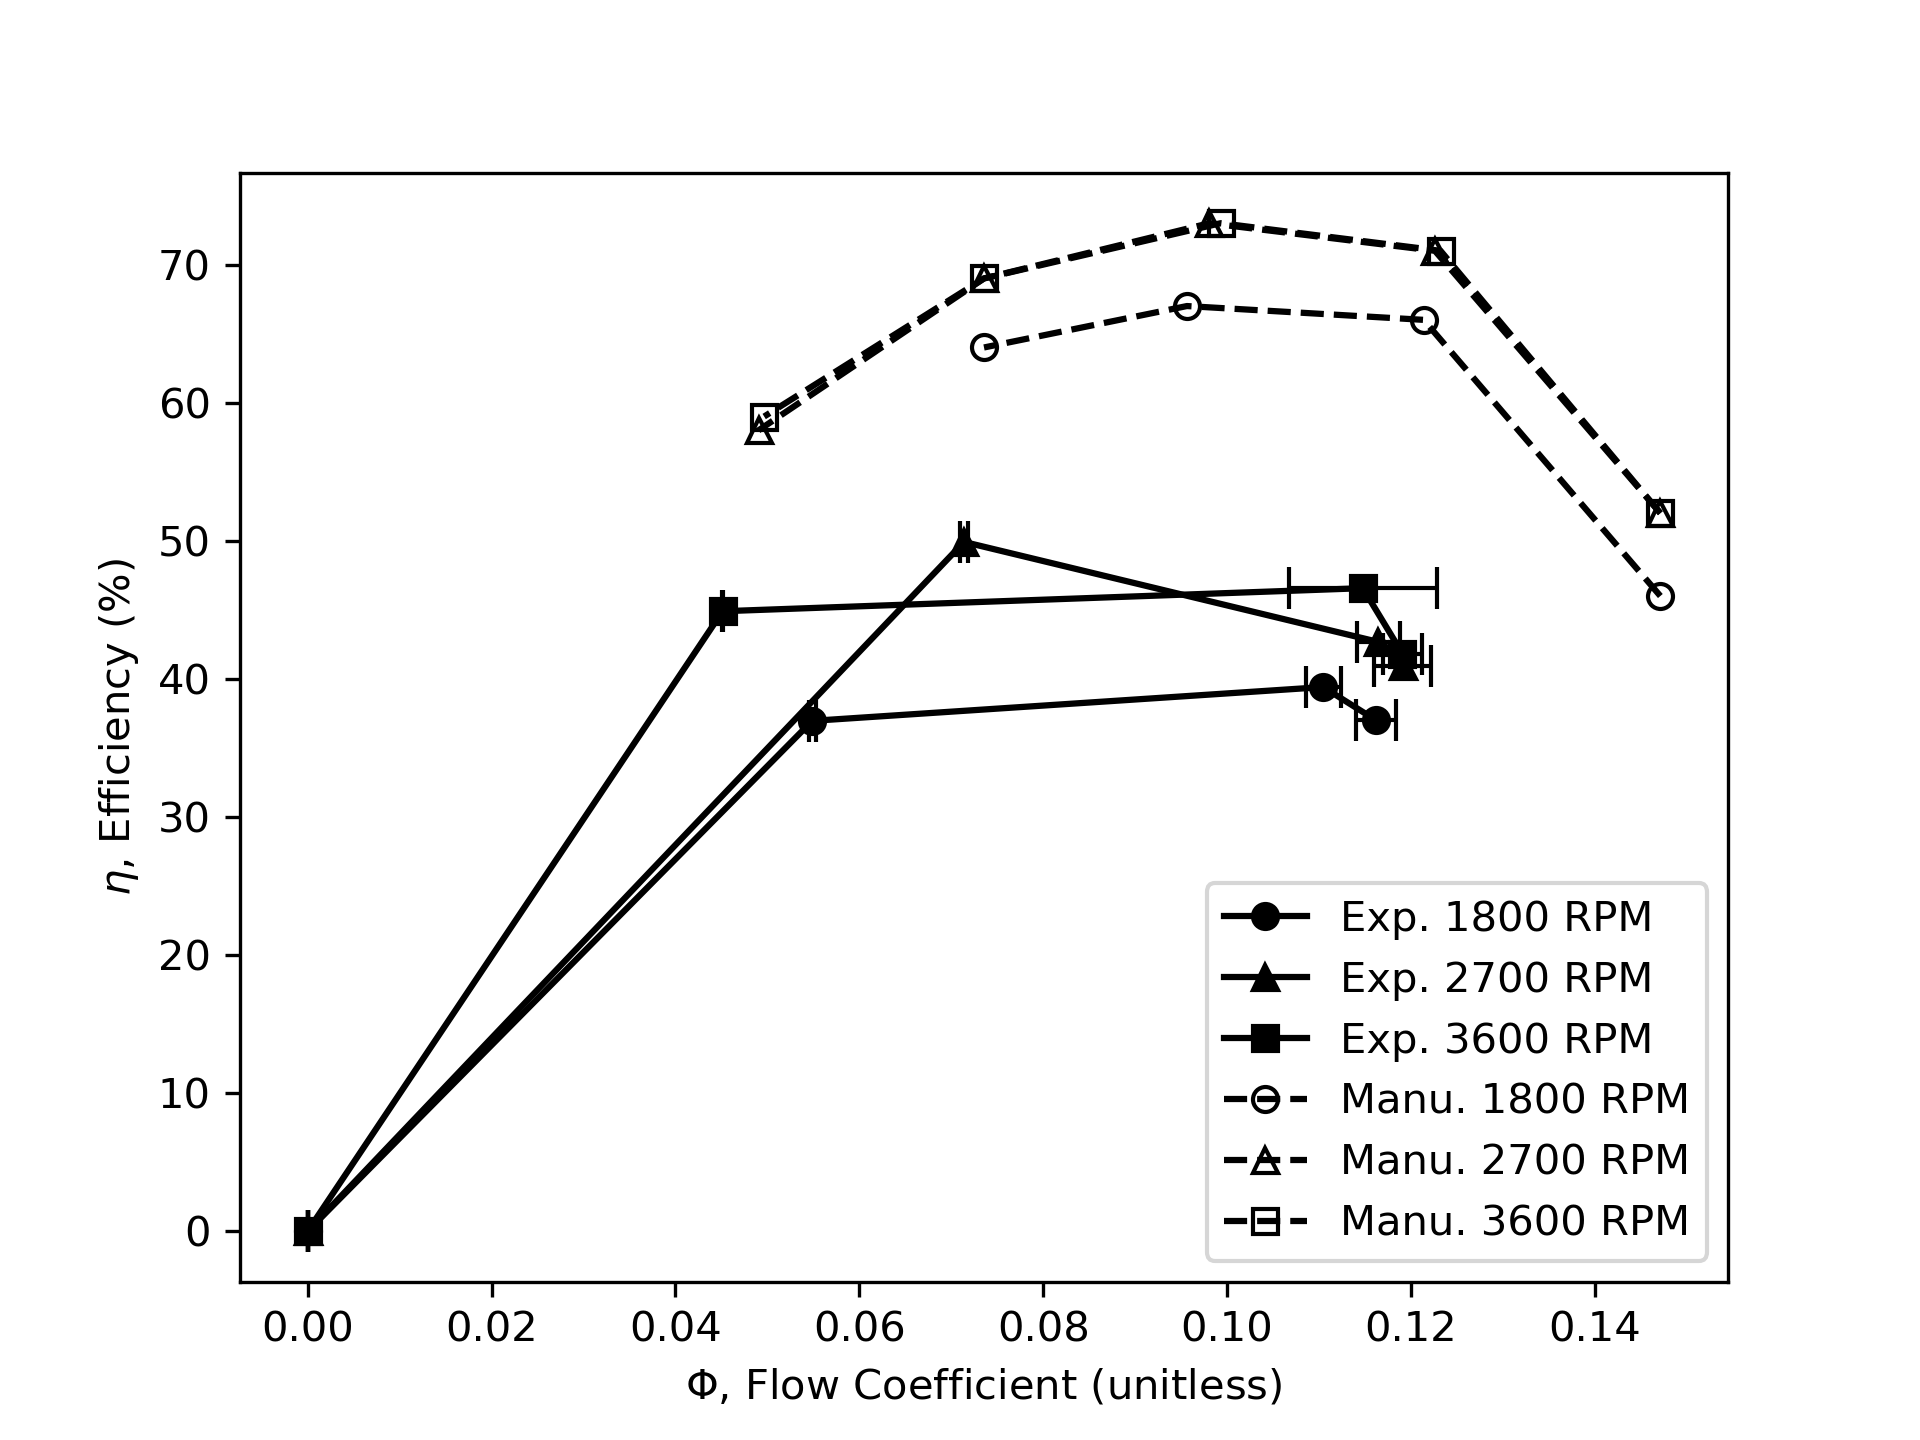
\includegraphics[width=0.5\textwidth]{Sections/Figures/Single Pump Efficiency Plot.png}
    \caption{Single pump experimental and manufacturer flow coefficient vs. efficiency plot.}
    \label{fig:single_pump_efficiency_plot}
\end{figure}

\subsection{Elevation Effects}
The vertical elevation of the pump lines have an effect on the head of the pump. This variation was not accounted for in the modelling. The transducers did not measure pressure immediately at the outlet due to the flow needing to develop fully. Some distance from the inlet was required due to the pressure gradient in the pump.

The error caused by the vertical displacements between the inlet and outlet was less than 0.2m (see Fig.\ref{fig:experimental_setup}). This would have added a small error of 0.2m to the head which is 2.6\% of the average head measured in the single pump configuration, 9.25m. This is a small error and was neglected.